% One-site TDVP, the backward half of a step: the effective Hamiltonian of
% the bond, applied to the centre after it has been split off the site.
%
% After AC is evolved it is factored, AC = AL C, AL joins the left
% environment, and the centre is C, on the bond. C carries no physical index,
% so nothing of the Hamiltonian sits here: the MPO's bond runs straight from L
% to R, which is the `-' slot -- a layer whose index passes through. C is then
% evolved backwards in time by this picture, and absorbed into the next site.
%
% The slot is the same width as a site's. The centre on a bond is a different
% shape (the small diamond) rather than a different slot.
\documentclass[border=4pt]{standalone}
\usepackage{amsmath,amssymb}
\usepackage{tikz-tensors}
\begin{document}
\begin{tikzpicture}
  \tnstack[left=$L$, right=$R$]{K}{1}{ket, op, bra}
  \tnlayer{K}{ket}{centrebond/$C$}
  \tnlayer{K}{op}{-}
  \tnconnect{K}
  \tnput[below]{K-left-bra}{$a$}
  \tnput[below]{K-right-bra}{$b$}
\end{tikzpicture}
\end{document}
